\documentclass[a4paper]{article}

\usepackage[english]{babel}
\usepackage[utf8]{inputenc}
\usepackage{amsmath}
\usepackage{graphicx}
\usepackage[colorinlistoftodos]{todonotes}
\usepackage{cite}
\usepackage{float}
\usepackage{hyperref}

\usepackage{footnote}
\makesavenoteenv{tabular}
\makesavenoteenv{table}

\title{Introducción a la ciencia de datos}

\author{Manuel Felipe Pineda L ~ 1093223607}

\date{\today}

\begin{document}
\maketitle
\begin{abstract}
  \noindent In this lab I will try to train a system with given
  metadata for emails sent to users in order to predict whether
  or not a future email will be opened for each user.

%  This metadata contains specific information about:
%
  %\begin{itemize}
    %\item The user the email was sent to.
    %\item The email that was sent.
    %\item The user's reaction to the email, including
      %(among other things) whether or not the user
      %opened the email.
  %\end{itemize}

  \noindent The data set contains 53 features for 486048 users.

  \noindent The project is based in a real competition that can be found
  \href{https://www.hackerrank.com/contests/machine-learning-codesprint/challenges/hackerrank-predict-email-opens}{here}

\end{abstract}

\section{Data attributes}

The attributes are fully described in the file ``attributes.pdf'',
and they are divided in four main sections.

\begin{description}
  \item [Contest logins] The attributes in this section have to do
    with the number of contests that a user actually logged in to
    HackerRank to compete in.
  \item [Contest Participation] The attributes in this section have
    to do with the number of contests that a user signed up for.
  \item [Account Information] This section contains miscellaneous
    attributes associated with a user’s account and their
    participation in the HackerRank community.
  \item [Email Attributes] This section contains attributes
    associated with emails sent to a user.
\end{description}

\section{Experiments}

For each experiment I used the classification report provided
in scikit-learn \cite{scikit-learn}, I also used the cross-validation
technique with the k-fold method, with k equals to ten, to evaluate the
estimators performance.

Each experiment was evaluated based in the f1-score and the
accuracy-score, were run in 4 cores \footnote{Intel(R) Core(TM)
i5-4300U CPU and 4 GB of RAM} and all were tested using
the methods ``fit'' and ``predict'' provided by the scikit-learn
API \cite{sklearn-api}.

\section{Visualization}

I used Principal Component Analysis (PCA) as dimensionality
reduction in order to plot the data, I also used Kernel PCA
as non-linear dimensionality reduction to see if it is able
to find a projection of the data that makes data linearly separable.

The figure \ref{fig:pca} shows that the data is not linearly separable
but give us information about the groups of users in the platform,
which could be very useful for other applications. In the figure
\ref{fig:kpca} we can observe how the transformations could help
to solve the problem making the classes more separable.

\begin{figure}
  \centering
  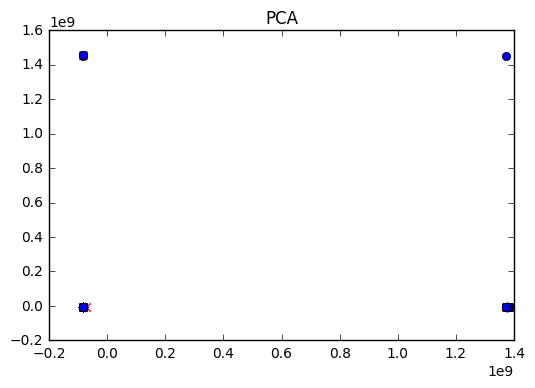
\includegraphics[width=0.6\textwidth]{./img/pca.png}
  \caption{\label{fig:pca} PCA}
\end{figure}

\begin{figure}
  \centering
  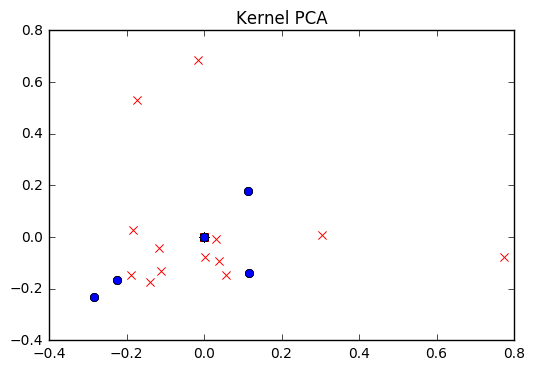
\includegraphics[width=0.6\textwidth]{./img/kpca.png}
  \caption{\label{fig:kpca} Kernel - PCA}
\end{figure}


\section{Estimators}

\subsection{Random guess}
I use a random guess to get a lower bound and evaluate the estimators.
\begin{verbatim}
Accuracy: 0.50 (+/- 0.00)
F1 score: 0.40 (+/- 0.00)
\end{verbatim}

The table \ref{tab:estimators} contains the evaluation of the estimators
with the default hyperparameters in order to compare them.

\begin{table}[]
\centering
\caption{Comparison between estimators}
\label{tab:estimators}
\begin{tabular}{llll}
\hline
\multicolumn{1}{l}{\textbf{Method}} & \multicolumn{1}{l}{\textbf{Accuracy}} & \multicolumn{1}{l}{\textbf{F1 Score}} & \multicolumn{1}{l}{\textbf{Time (s)}} \\ \hline
\textbf{Linear models} & & & \\ \hline
Perceptron & 0.60 (+/- 0.35) & 0.37 (+/- 0.21) & 15.18  \\
Logistic Regression & 0.72 (+/- 0.00) & 0.28 (+/- 0.01) & 68.48 \\
Stochastic GD & 0.68 (+/- 0.23) & 0.30 (+/- 0.25) & 15.49 \\
SGD log reg as loss & 0.60 (+/- 0.35) & 0.39 (+/- 0.22) & 15.78 \\
Passive Aggressive Classifier & 0.56 (+/- 0.38) & 0.37 (+/- 0.21) & 23.27 \\
\textbf{Non linear transformation} & & & \\ \hline
SVC & 0.67 (+/- 0.01) & 0.02 (+/- 0.02) & 28.05 \\
NuSVC & 0.67 (+/- 0.00) & 0.01 (+/- 0.02) & 29.39 \\
Random Trees Embbedings & 0.72 (+/- 0.00) & 0.28 (+/- 0.01) & 141.27 \\
Extra Trees Classifier \footnote{This classifier is able to
get perfect score using the whole data set}
& 0.70 (+/- 0.03) & 0.41 (+/- 0.06) & 1.25 \\
Naive Bayes & 0.68 (+/- 0.00) & 0.41 (+/- 0.01) & 41.89 \\
RBF Sampler (Kernel approx) & 0.64 (+/- 0.03) & 0.16 (+/- 0.08)
& 1.54 \\
\textbf{Manifold Learning} & & & \\ \hline
K Neighbors Classifier & 0.61 (+/- 0.04) & 0.41 (+/- 0.05) & 1.58 \\
Radius Neighbors Classifier & 0.67 (+/- 0.00) & 0.00 (+/- 0.00) & 12.97 \\
\textbf{ANN} & & & \\ \hline
Multilayer Perceptron & 0.33 (+/- 0.00) & 0.50 (+/- 0.00) & 11.18 \\
\end{tabular}
\end{table}

\section{Tuning hyperparameters}

I used the Exhaustive Grid Search to optimize best the classifiers.


\noindent The best parameters with KFold and cross validation
under the f1 score are the following:

\subsection{Optimizing Multilayer Perceptron}

\begin{verbatim}
{
  'tol': 1e-05,
  'activation': 'identity',
  'alpha': 1.0,
  'learning_rate': 'adaptive',
  'hidden_layer_sizes': (100, 33),
  'solver': 'lbfgs',
  'max_iter': 400
}
\end{verbatim}
With f1 score of 0.50, done in 11507.70 s

\subsection{Optimizing K Neighbors}
\begin{verbatim}

{
  'weights': 'uniform',
  'n_neighbors': 1
}
\end{verbatim}
With f1 score of 0.41, done in 40.58 s
\subsection{Optimizing Extra Trees Classifier}
\begin{verbatim}
{
  'class_weight': 'balanced_subsample',
  'max_depth': None,
  'n_estimators': 1024,
  'min_samples_split': 256
}
\end{verbatim}

With f1 score of 0.51, done in 1698.70 s

\section{Results}

The current data is very complex, as result, most of the
classifiers get bad performance, even worse that random. However,
it is possible to configure some estimators in order to receive
better score that pure chance.

This process is very demanding in terms of time and processing because
needs to explore a wide range of hyperparameters and the execution
becomes exponential in the number of hyperparameters.

By the way, if we compare the score with respect the official
leaderboard for the contest, this solution would result in the
place 80 of 500.

\bibliography{mybib}{}
\bibliographystyle{unsrt}

\end{document}

